% Bozza M13.5: sezioni indipendenti dai nuovi risultati sperimentali.
% Da inserire in main.tex al posto delle attuali sezioni 2, 3.2, 4 (parte astratta), 5, 6.
% I punti ancora da riempire con dati del 13.3-bis/13.4 sono marcati con \todo{...}.
\documentclass[11pt,a4paper]{article}
\usepackage[utf8]{inputenc}
\usepackage[T1]{fontenc}
\usepackage[english]{babel}
\usepackage[margin=2.3cm]{geometry}
\usepackage{amsmath,amssymb,booktabs,graphicx,hyperref,caption,enumitem,float,xcolor}
\usepackage{algorithm}
\usepackage{algpseudocode}
\usepackage{tikz}
\usetikzlibrary{arrows.meta,positioning,shapes.geometric,fit,calc}
\newcommand{\todo}[1]{\textcolor{red}{[TODO: #1]}}
\captionsetup{font=small}
\begin{document}

\section{Problem and sequential algorithm}

The workload is the verification of ECDSA signatures on the NIST P-256 curve. The input is a batch of $N$ records; each record holds a public key $Q$, a message $m$ and a signature $(r,s)$. The output is the number of records whose signature is valid. The batch has no internal order and the records do not depend on each other.

\subsection{Verification of one signature}

Let $G$ be the base point of the curve, $n$ its prime order, and $H$ the SHA-256 hash. Verifying one record means the following steps.

\begin{algorithm}[H]
\caption{Verification of one ECDSA signature (sequential)}
\begin{algorithmic}[1]
\Require public key $Q$, message $m$, signature $(r,s)$
\Ensure \textsc{valid} or \textsc{invalid}
\If{$r\notin[1,n-1]$ \textbf{or} $s\notin[1,n-1]$} \Return \textsc{invalid} \EndIf
\State $e \gets H(m)$ interpreted as an integer
\State $w \gets s^{-1} \bmod n$
\State $u_1 \gets e\,w \bmod n,\quad u_2 \gets r\,w \bmod n$
\State $R \gets u_1 G + u_2 Q$ \Comment{two scalar multiplications on the curve}
\If{$R$ is the point at infinity} \Return \textsc{invalid} \EndIf
\State \Return \textsc{valid} \textbf{if} $x_R \bmod n = r$, else \textsc{invalid}
\end{algorithmic}
\end{algorithm}

In the code this sequence is one call pair to the OpenSSL EVP interface (\texttt{EVP\_DigestVerifyInit} with SHA-256 on the EC key, then \texttt{EVP\_DigestVerify}), not a direct call to \texttt{ECDSA\_verify}. The scalar multiplications in step 5 are where the time goes: the profile in Section~\ref{sec:profile} puts more than 85\% of the executed instructions in modular arithmetic on field and group elements.

\subsection{Sequential benchmark}

\begin{algorithm}[H]
\caption{Sequential batch verification (reference solution, time $T_1$)}
\begin{algorithmic}[1]
\Require batch of $N$ records
\State $\textit{valid} \gets 0$
\For{$i = 0,\dots,N-1$}
  \State allocate a verification context
  \If{\textsc{Verify}$(\text{record}_i)$ is valid} $\textit{valid} \gets \textit{valid}+1$ \EndIf
  \State release the context
\EndFor
\State check that $\textit{valid} = N$ \Comment{all synthetic signatures are valid by construction}
\State \Return \textit{valid}
\end{algorithmic}
\end{algorithm}

The time $T_1$ of this loop on one thread, compiled with \texttt{-O2}, is the denominator of every speedup in this report. It excludes the generation of the synthetic dataset and the start-up of the process. \todo{cost of one verification: mean, standard deviation, coefficient of variation, p99, from per\_verify\_cost.csv (stage 13.4, B0)}

\begin{figure}[H]
\centering
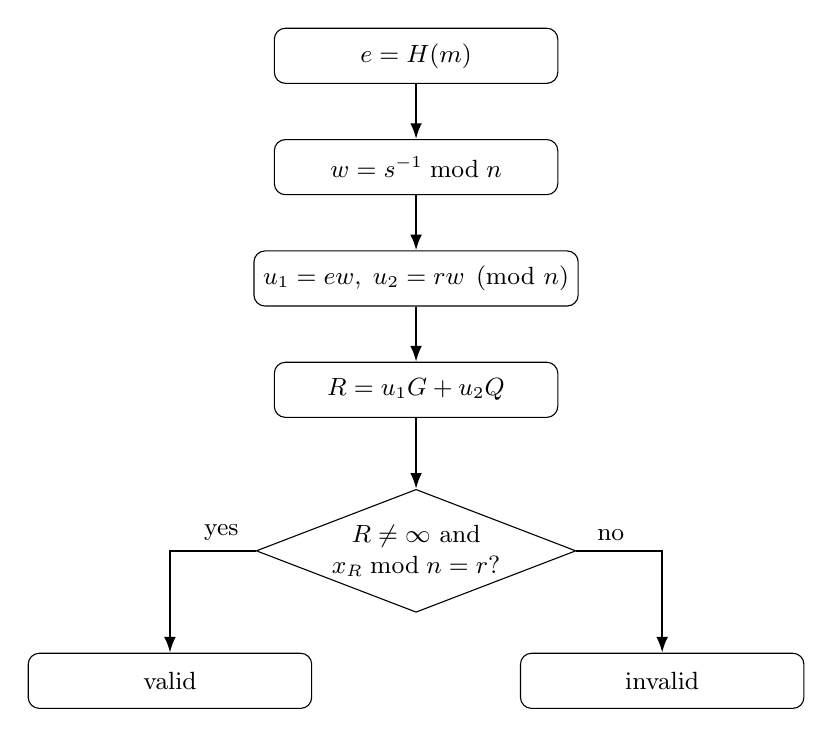
\begin{tikzpicture}[node distance=0.7cm, every node/.style={font=\small},
  box/.style={draw,rounded corners,minimum width=3.6cm,minimum height=0.7cm,align=center},
  dec/.style={draw,diamond,aspect=2.6,inner sep=1pt,align=center},
  arr/.style={-{Latex[length=2mm]},thick}]
\node[box] (a) {$e = H(m)$};
\node[box,below=of a] (b) {$w = s^{-1} \bmod n$};
\node[box,below=of b] (c) {$u_1 = e w,\; u_2 = r w \pmod n$};
\node[box,below=of c] (d) {$R = u_1 G + u_2 Q$};
\node[dec,below=0.9cm of d] (e) {$R \ne \infty$ and\\$x_R \bmod n = r$?};
\node[box,below left=0.9cm and 0.3cm of e] (v) {valid};
\node[box,below right=0.9cm and 0.3cm of e] (i) {invalid};
\draw[arr] (a)--(b); \draw[arr] (b)--(c); \draw[arr] (c)--(d); \draw[arr] (d)--(e);
\draw[arr] (e)-|node[above,pos=0.2]{yes}(v);
\draw[arr] (e)-|node[above,pos=0.2]{no}(i);
\end{tikzpicture}
\caption{Flow of one verification, after the range check on $r$ and $s$.}
\end{figure}

\subsection{Profile of the sequential code}\label{sec:profile}
\todo{keep the existing Section 3.1 text and Table 1; change ``of the total time'' to ``of the executed instructions'', since Callgrind counts instructions and not time.}

\section{Partitioning}\label{sec:partitioning}

This section describes the decomposition of the problem into tasks. It does not depend on how the tasks are later executed: no process, thread or message appears here.

\subsection{Tasks and data}

\begin{itemize}[nosep]
  \item \textbf{Verification task} $V_i$, for $i=0,\dots,N-1$. Input: record $i$. Output: one bit $b_i\in\{0,1\}$. This is the finest useful task; it is a single call of Algorithm~1.
  \item \textbf{Reduction task} $\Sigma$. Input: the $N$ bits. Output: $\sum_i b_i$.
\end{itemize}

The data domain is the batch, and the decomposition is a domain decomposition: every $V_i$ applies the same operation to a different record. There are $N$ verification tasks and one reduction task, with $N$ much larger than the number of processing elements used in the experiments ($N=20{,}000$ against at most 20 or 32 elements).

\subsection{Task dependency graph}

\begin{figure}[H]
\centering
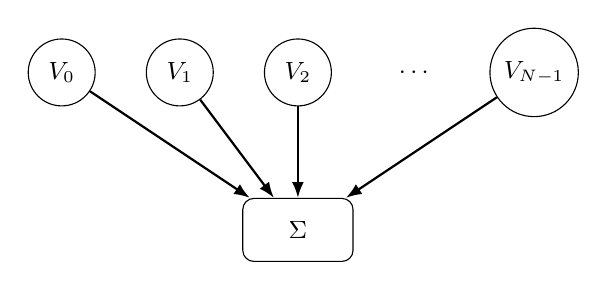
\begin{tikzpicture}[every node/.style={font=\small},
  t/.style={draw,circle,minimum size=0.85cm},
  s/.style={draw,rounded corners,minimum width=1.4cm,minimum height=0.8cm},
  arr/.style={-{Latex[length=2mm]},thick}]
\foreach \i/\l in {0/{V_0},1/{V_1},2/{V_2},4/{V_{N-1}}} {
  \node[t] (v\i) at (\i*1.5,0) {$\l$};
}
\node at (4.5,0) {$\cdots$};
\node[s] (r) at (3,-2) {$\Sigma$};
\foreach \i in {0,1,2,4} \draw[arr] (v\i)--(r);
\end{tikzpicture}
\caption{Task dependency graph of the batch: $N$ independent verification tasks and one reduction that depends on all of them. The critical path has length two.}
\end{figure}

The verification tasks have no dependency among themselves. Their dependency edges all end at $\Sigma$, so the maximum degree of concurrency is $N$ and the length of the critical path is one verification plus one reduction.

\subsection{Task interaction graph}

The verification tasks do not exchange data during execution, so the interaction graph has no edge between two $V_i$. The only interaction is the final one with $\Sigma$, and it carries one integer per contributing group of tasks. The interaction is therefore static, regular and read-once.

\subsection{A second decomposition: the three-stage chain}

The production platform also contains a functionally decomposed workload: three stages $S_1\to S_2\to S_3$, where the output of one stage is the input of the next.

\begin{figure}[H]
\centering
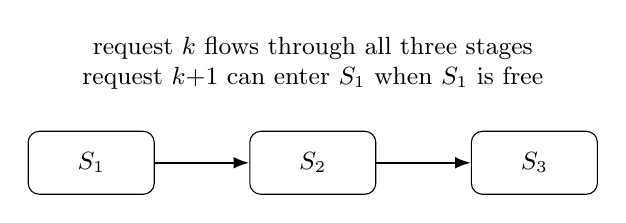
\begin{tikzpicture}[every node/.style={font=\small},
  s/.style={draw,rounded corners,minimum width=1.6cm,minimum height=0.8cm},
  arr/.style={-{Latex[length=2mm]},thick}]
\node[s] (a) {$S_1$}; \node[s,right=1.2cm of a] (b) {$S_2$}; \node[s,right=1.2cm of b] (c) {$S_3$};
\draw[arr] (a)--(b); \draw[arr] (b)--(c);
\node[above=0.4cm of b,align=center] {request $k$ flows through all three stages\\request $k{+}1$ can enter $S_1$ when $S_1$ is free};
\end{tikzpicture}
\caption{Dependency and interaction graph of the chain. Both graphs are the same path, because each stage depends on and communicates with only its predecessor.}
\end{figure}

Unlike the batch, this decomposition has a real data dependency, so within one request the three stages cannot overlap. Overlap is possible only across different requests, which is what the pipelining experiment measures.

\section{Communication, agglomeration and aggregation}

\subsection{Data that must move}

In the batch decomposition a task needs no input transfer: the records are generated deterministically from a seed at the processing element that verifies them, so only the seed, the batch size and the thread count are passed as parameters. The only data that flows back is an integer (the number of valid signatures) and a time value per group of tasks. The volume exchanged is therefore a few bytes per group, independent of $N$. \todo{state per substrate (MPI, gRPC, IoTronic chain) what is sent, using Table 2 of the current report}

\subsection{Agglomeration}

Running one task per message or per call would make the overhead per task comparable to the task itself. The tasks are agglomerated into chunks of consecutive records. With $P$ groups and $N$ records, group $g$ gets
\[
n_g = \left\lfloor \frac{N}{P} \right\rfloor + \begin{cases}1 & g < N \bmod P\\0 & \text{otherwise,}\end{cases}
\]
so sizes differ by at most one record. Agglomeration happens at two levels: the batch is first split into $P$ chunks (one per process or node), and each chunk is split again among the threads of that process. The same remainder rule is used in the MPI code and in the gRPC dispatcher.

\subsection{Aggregation}
\todo{keep the current Section 5; add one sentence for the new master-worker variant: the master sums the partial counts it receives, and workers report their maximum compute time through a reduction.}

\section{Mapping}\label{sec:mapping}

Mapping assigns the agglomerated chunks to processing elements. The table lists the policy used in each setting; it separates the decision about \emph{which} element runs a chunk from the decision about \emph{when} the assignment is made.

\begin{table}[H]
\centering\small
\begin{tabular}{p{3.2cm}p{2.4cm}p{4.2cm}p{4.2cm}}
\toprule
\textbf{Setting} & \textbf{Static / dynamic} & \textbf{Policy} & \textbf{Reason} \\
\midrule
OpenMP loop (threads) & static by default; dynamic and guided measured & \texttt{schedule(runtime)}, default set to static unless \texttt{OMP\_SCHEDULE} is defined & the cost of one verification is nearly uniform \todo{CV from B0}; E5 tests whether a dynamic schedule changes anything \\
MPI, statically partitioned & static & block partition with remainder, one chunk per rank, decided before the run & no communication is needed during the run; imbalance is at most one record \\
MPI master-worker & dynamic & rank 0 hands a chunk to whichever worker asks next; chunk size is a parameter & absorbs unequal speeds between workers; costs one message per chunk and a coordinator that does not compute \\
OpenMP \texttt{taskloop} & dynamic & tasks of \texttt{grainsize} iterations taken from a shared queue by idle threads & task-based version of the same loop \\
gRPC dispatch (isolated benchmark) & static & block partition with remainder; chunk $g$ goes to worker $g$ & workers are identical containers on one host \\
Production chain (IoTronic) & dynamic selection, static split & the set of nodes is chosen at lease time among online boards approved on-chain (first fit); then the batch is split in blocks in lease order & boards can appear or disappear between requests, so the node set cannot be fixed in advance \\
\bottomrule
\end{tabular}
\caption{Mapping policy for each setting.}
\end{table}

\subsection{Mapping to hardware}

\todo{from stage 13.3-bis A3: table of experiment / ranks / threads / binding flags / cpuset, with the number of OpenMP threads of one rank that share a physical core and whether two ranks share a core. Write what was actually used: the launch scripts use \texttt{--use-hwthread-cpus} and \texttt{--bind-to hwthread}, not \texttt{--bind-to core}, in the final campaign.}

The machine has six performance cores with two hardware threads each (logical CPUs 0--11) and eight efficiency cores with one thread each (logical CPUs 12--19). The configurations that stay within CPUs 0--11 are separated from the others in the plots, and experiment E8 repeats pure OpenMP and pure MPI restricted to CPUs 0--11 to check whether the core type changes the curves. \todo{result of E8, only after stage 13.4}

\subsection{Static against dynamic mapping}
\todo{after stage 13.4: result of E5 (OpenMP schedules) and E6 (master-worker, taskloop). If the interquartile ranges overlap, say that no difference was measured.}

\section{Hybrid implementation: processes and threads}

The hybrid program has two levels of parallelism, and each level has its own mechanism.

\begin{figure}[H]
\centering
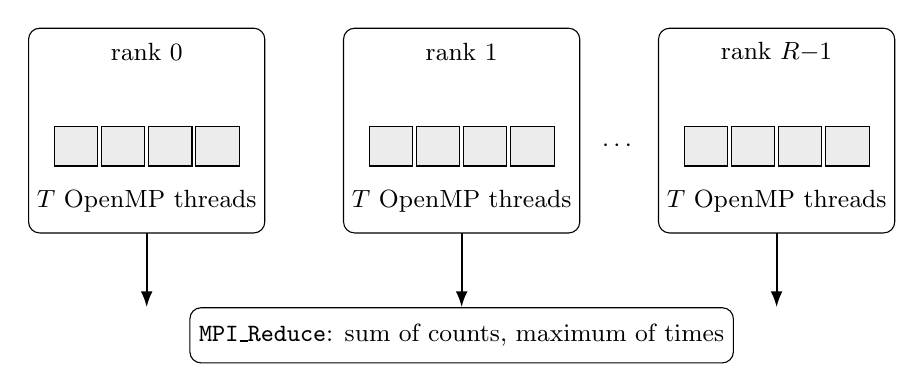
\begin{tikzpicture}[every node/.style={font=\small},
  proc/.style={draw,rounded corners,minimum width=3.0cm,minimum height=2.6cm,align=center},
  th/.style={draw,minimum width=0.55cm,minimum height=0.5cm,fill=gray!15},
  arr/.style={-{Latex[length=2mm]},thick}]
\node[proc] (p0) at (0,0) {};
\node[proc] (p1) at (4,0) {};
\node[proc] (p2) at (8,0) {};
\node at (0,1.0) {rank 0}; \node at (4,1.0) {rank 1}; \node at (8,1.0) {rank $R{-}1$};
\foreach \x in {0,4,8}{
  \foreach \k in {-0.9,-0.3,0.3,0.9} \node[th] at (\x+\k,-0.2) {};
  \node at (\x,-0.9) {$T$ OpenMP threads};
}
\node at (6,-0.2) {$\cdots$};
\node[draw,rounded corners,minimum width=6.5cm,minimum height=0.7cm] (red) at (4,-2.6) {\texttt{MPI\_Reduce}: sum of counts, maximum of times};
\foreach \x in {0,4,8} \draw[arr] (\x,-1.3)--(red.north -| \x,0);
\end{tikzpicture}
\caption{Two levels: $R$ MPI processes, each running $T$ threads in a parallel loop over its own chunk. MPI is called only by the master thread of each process, outside the parallel region.}
\end{figure}

\begin{itemize}[nosep]
  \item \textbf{Inter-process level.} The batch is split into $R$ chunks with the remainder rule above. Each rank verifies its own chunk and the results are combined with two reductions: a sum for the number of valid signatures and a maximum for the elapsed time, because the slowest rank decides when the whole job ends.
  \item \textbf{Intra-process level.} Inside a rank, the chunk is verified by an OpenMP parallel loop with a reduction on the valid counter. The number of threads $T$ is a command-line parameter. Each iteration allocates its own verification context, so threads share no mutable state except the counter that OpenMP reduces.
  \item \textbf{Interface between the two.} MPI is initialised with \texttt{MPI\_Init\_thread} requesting \texttt{MPI\_THREAD\_FUNNELED}, and the program aborts if the library grants less. No MPI call is made inside the parallel region, so this level is enough.
  \item \textbf{The same two levels in the distributed setting.} A gRPC worker receives \texttt{num\_threads} in the request and runs the same OpenMP loop. The dispatcher plays the role of the MPI reduction: it sums the partial counts and checks that the total equals the batch size.
\end{itemize}

The effective parallelism of a configuration is $P_{\mathrm{eff}} = R\times T$. \todo{binding used for each configuration, from Section 6.1 above.}

\end{document}